\documentclass[a4paper,12pt]{article}
\usepackage[utf8]{inputenc}
\usepackage[german]{babel}
\usepackage{amsmath}
\usepackage{amssymb}
\usepackage{amsthm}
\usepackage{geometry}
\usepackage{graphicx}
\usepackage[hidelinks]{hyperref}
\usepackage{listings}
\usepackage{xcolor}
\usepackage{enumitem}
\usepackage{microtype}
\usepackage{booktabs}
\usepackage{array}
\usepackage{url}

% Prevent all overflows
\sloppy
\emergencystretch=3em
\hbadness=10000
\hfuzz=2pt
\Urlmuskip=0mu plus 2mu

\geometry{margin=2.5cm}

\theoremstyle{definition}
\newtheorem{definition}{Definition}
\newtheorem{beispiel}{Beispiel}
\newtheorem{satz}{Satz}
\newtheorem{lemma}{Lemma}
\newtheorem{bemerkung}{Bemerkung}

\setlist[itemize,1]{label=--}

% ---------- Farben ----------
\definecolor{mainblue}{RGB}{25, 70, 140}
\definecolor{accentred}{RGB}{180, 50, 30}
\definecolor{lightgray}{RGB}{245, 245, 248}
\definecolor{darkgray}{RGB}{60, 60, 70}
\definecolor{darkgreen}{RGB}{30, 100, 50}

\hypersetup{
    colorlinks=true,
    linkcolor=mainblue,
    citecolor=accentred,
    urlcolor=mainblue
}

%  Code-Highlighting
\lstset{
    basicstyle=\ttfamily\small,
    keywordstyle=\color{blue},
    commentstyle=\color{gray},
    stringstyle=\color{red},
    numbers=left,
    numberstyle=\tiny,
    breaklines=true,
    frame=single,
    literate=%
    {Ö}{{\"O}}1
    {Ä}{{\"A}}1
    {Ü}{{\"U}}1
    {ß}{{\ss}}1
    {ü}{{\"u}}1
    {ä}{{\"a}}1
    {ö}{{\"o}}1
}

\title{Funktionale Sicherheit nach ISO~26262:\\
Formale Grundlagen, ASIL-Klassifikation und\\
Verifikationsmethoden für Straßenfahrzeuge}
\author{Stephan Epp}
\date{25. Juni 2026}

\begin{document}

\maketitle

\tableofcontents
\newpage

% ═══════════════════════════════════════════════════════
\section{Einführung}
% ═══════════════════════════════════════════════════════

Die Norm ISO~26262 \emph{Road vehicles -- Functional Safety} ist der maßgebliche
internationale Standard für die funktionale Sicherheit elektrischer und
elektronischer (E/E-)~Systeme in Straßenfahrzeugen~\cite{iso26262_2018}.
Sie definiert einen systematischen Entwicklungsprozess, der sicherstellt,
dass E/E-Systeme auch im Fehlerfall keine unvertretbaren Risiken für Personen
erzeugen.

\subsection{Problemstellung}

Moderne Kraftfahrzeuge enthalten mehrere Hundert elektronische Steuergeräte
(ECUs), die über Bussysteme wie CAN, FlexRay oder Ethernet miteinander
kommunizieren. Fehlfunktionen in sicherheitskritischen Systemen -- etwa dem
Antiblockiersystem (ABS), dem elektronischen Stabilitätsprogramm (ESP) oder
dem autonomen Notbremsassistenten -- können zu schwerwiegenden Unfällen führen.

\textbf{Kernproblem:} Wie lässt sich für ein komplexes E/E-System
\emph{formal} nachweisen, dass es mit hinreichend hoher Zuverlässigkeit
die geforderten Sicherheitsziele erfüllt, selbst wenn zufällige Hardware\-fehler
oder systematische Entwicklungsfehler auftreten?

ISO~26262 beantwortet diese Frage durch:
\begin{itemize}
  \item eine risikoproportionale Klassifikation (ASIL~A bis ASIL~D),
  \item einen vollständigen Entwicklungslebenszyklus (V-Modell),
  \item quantitative Anforderungen an Hardwarezuverlässigkeit und
        Diagnoseabdeckung,
  \item formale Sicherheitsnachweise (Safety Cases).
\end{itemize}

\subsection{Motivation}

Die wirtschaftliche und gesellschaftliche Bedeutung der Norm ist erheblich.
Allein in der Europäischen Union forderten Straßenverkehrsunfälle im
Jahr~2022 rund 20\,400 Todesopfer~\cite{eu_road_safety_2023}. Studien der
National Highway Traffic Safety Administration (NHTSA) zeigen, dass mehr
als 20\,\% der Unfälle auf Fahrzeugtechnikversagen zurückzuführen
sind~\cite{nhtsa_2022}. Eine konsequente Anwendung von ISO~26262 kann
diesen Anteil signifikant reduzieren.

Darüber hinaus stellen Original Equipment Manufacturer (OEM) und
Tier-1-Zulieferer die Normenkonformität als juristischen Haftungsschutz
sicher. Für neue Fahrzeugbaureihen ist der Nachweis der
ISO~26262-Konformität in vielen Märkten Voraussetzung für die Typzulassung.

\subsection{Beitrag dieser Arbeit}

Diese Arbeit liefert:
\begin{enumerate}
  \item eine \emph{formale} mathematische Fundierung der zentralen Konzepte
        (ASIL-Klassifikation, Ausfallrate, Diagnoseabdeckung),
  \item vollständige Beweise der quantitativen Anforderungen,
  \item experimentell erzeugte Visualisierungen aller Kernzusammenhänge,
  \item einen ausführlichen Ausblick auf offene Forschungsfragen im Bereich
        Functional Safety und autonomes Fahren.
\end{enumerate}

% ═══════════════════════════════════════════════════════
\section{Grundlagen}
% ═══════════════════════════════════════════════════════

\subsection{Definitionen}

\begin{definition}[Schaden (Harm)]
  Ein \emph{Schaden} ist eine physische Verletzung oder Beeinträchtigung
  der Gesundheit von Personen. Die Norm unterscheidet Schweregrade
  $S \in \{0, 1, 2, 3\}$, wobei $S=0$ kein Verletzungspotenzial und
  $S=3$ lebensbedrohliche oder tödliche Verletzungen bezeichnet.
\end{definition}

\begin{definition}[Gefährdung (Hazard)]
  Eine \emph{Gefährdung} ist eine potenzielle Quelle eines Schadens,
  die durch eine Fehlfunktion eines E/E-Systems verursacht werden kann.
  Formal: Eine Gefährdung $h$ ist ein Paar $(f, s)$ bestehend aus einer
  Fehlfunktion $f$ und einer Betriebssituation $s$.
\end{definition}

\begin{definition}[Exposition (Exposure)]
  Die \emph{Exposition} $E \in \{0, 1, 2, 3, 4\}$ beschreibt die
  Häufigkeit, mit der ein Fahrzeug in eine Betriebssituation gerät,
  in der eine Gefährdung zu einem Schaden führen kann:
  \[
    E = \begin{cases}
      0 & \text{unglaublich selten} \\
      1 & \text{sehr selten (weniger als einmal pro Jahr)} \\
      2 & \text{selten (einige Male pro Jahr)} \\
      3 & \text{gelegentlich (einige Male pro Monat)} \\
      4 & \text{häufig (täglich oder öfter)}
    \end{cases}
  \]
\end{definition}

\begin{definition}[Kontrollierbarkeit (Controllability)]
  Die \emph{Kontrollierbarkeit} $C \in \{0, 1, 2, 3\}$ beschreibt die
  Möglichkeit des Fahrers, einen Unfall bei Auftreten der Gefährdung
  zu vermeiden:
  \[
    C = \begin{cases}
      0 & \text{allgemein kontrollierbar} \\
      1 & \text{einfach kontrollierbar (über 99\,\%)} \\
      2 & \text{normal kontrollierbar (über 90\,\%)} \\
      3 & \text{schwer kontrollierbar (unter 90\,\%)}
    \end{cases}
  \]
\end{definition}

\begin{definition}[Automotive Safety Integrity Level (ASIL)]
  Der \emph{ASIL} ist ein risikobasierter Sicherheitsgrad
  $\mathrm{ASIL} \in \{\text{QM}, \text{A}, \text{B}, \text{C}, \text{D}\}$,
  der aus den Parametern Schwere $S$, Exposition $E$ und
  Kontrollierbarkeit $C$ abgeleitet wird.
  $\mathrm{QM}$ (Quality Management) bedeutet, dass keine speziellen
  funktionalen Sicherheitsanforderungen notwendig sind.
\end{definition}

\begin{definition}[Sicherheitsziel (Safety Goal)]
  Ein \emph{Sicherheitsziel} ist eine übergeordnete Sicherheitsanforderung
  an ein Item, die das Auftreten einer Gefährdung verhindert oder deren
  Auswirkung auf einen tolerierbaren Schaden begrenzt.
  Jedem Sicherheitsziel wird ein ASIL zugewiesen.
\end{definition}

\begin{definition}[Ausfallrate und FIT]
  Die \emph{Ausfallrate} $\lambda$ eines Bauteils wird in der Einheit
  \emph{FIT} (Failure In Time) angegeben:
  \[
    1\;\mathrm{FIT} = 10^{-9}\;\text{Ausfälle pro Betriebsstunde.}
  \]
  Für ein exponentialverteiltes Bauteil gilt die Zuverlässigkeitsfunktion
  $R(t) = e^{-\lambda t}$, wobei $\lambda$ die konstante Ausfallrate ist.
\end{definition}

\begin{definition}[Diagnoseabdeckung (Diagnostic Coverage, DC)]
  Die \emph{Diagnoseabdeckung} $\mathrm{DC}$ ist der Anteil der durch
  Sicherheitsmechanismen erkannten gefährlichen Ausfälle:
  \[
    \mathrm{DC}
    = \frac{\lambda_{\mathrm{DD}}}{\lambda_{\mathrm{D}}}
    = \frac{\lambda_{\mathrm{D}} - \lambda_{\mathrm{DU}}}{\lambda_{\mathrm{D}}},
  \]
  wobei $\lambda_{\mathrm{DD}}$ die Rate erkannter und
  $\lambda_{\mathrm{DU}}$ die Rate unerkannter gefährlicher Ausfälle
  bezeichnen.
\end{definition}

\begin{definition}[Probabilistic Metric for Hardware Failure (PMHF)]
  Die \emph{PMHF} ist der Gesamtbeitrag aller Hardwareausfälle zur
  Verletzung eines Sicherheitsziels pro Betriebsstunde:
  \[
    \mathrm{PMHF}
    = \sum_{i} \lambda_{\mathrm{DU},i}
    + \sum_{j} \lambda_{\mathrm{S},j} \cdot (1 - \mathrm{DC}_j),
  \]
  wobei über alle Einzelfehlerquellen $i$ und latente Mehrfachfehler
  $j$ summiert wird.
\end{definition}

\subsection{Grundidee der ASIL-Klassifikation}

\subsubsection{Risikograph}

Die ASIL-Einstufung folgt dem Risikographen nach ISO~26262-3:5.4.
Der risikoproportionale Zusammenhang lässt sich durch eine
Bewertungsfunktion formalisieren.

\begin{satz}[ASIL-Bestimmungsfunktion]
\label{satz:asil_funktion}
  Die ASIL-Einstufung $\mathrm{ASIL}(S, E, C)$ ist eine monoton
  wachsende Funktion in $S$, $E$ und $C$. Formal existiert eine
  streng monotone Ordnung
  $\mathrm{QM} \prec \mathrm{A} \prec \mathrm{B} \prec \mathrm{C}
  \prec \mathrm{D}$, sodass für alle zulässigen Parameter gilt:
  \[
    S' \geq S,\; E' \geq E,\; C' \geq C
    \;\implies\;
    \mathrm{ASIL}(S', E', C') \succeq \mathrm{ASIL}(S, E, C).
  \]
\end{satz}

\begin{proof}
  Die ASIL-Klassifikation ist in ISO~26262-3, Tabelle~4 als vollständige
  Entscheidungsmatrix definiert. Eine Inspektion dieser Tabelle zeigt:
  \begin{itemize}
    \item Erhöhung von $S$ bei festem $(E, C)$ führt nie zu einem
          niedrigeren ASIL.
    \item Erhöhung von $E$ bei festem $(S, C)$ führt nie zu einem
          niedrigeren ASIL.
    \item Erhöhung von $C$ bei festem $(S, E)$ führt nie zu einem
          niedrigeren ASIL.
  \end{itemize}
  Ein höheres Risiko (größere Schwere, häufigere Exposition oder
  schwierigere Kontrollierbarkeit) erfordert eine strengere
  Sicherheitsanforderung. Die Monotonie folgt direkt aus dem
  Risikoabbau-Prinzip der Norm (ISO~26262-3:5.4.3).
\end{proof}

Abbildung~\ref{fig:asil_matrix} visualisiert die ASIL-Risikomatrix
für den repräsentativen Fall $C=3$.

\begin{figure}[ht]
  \centering
  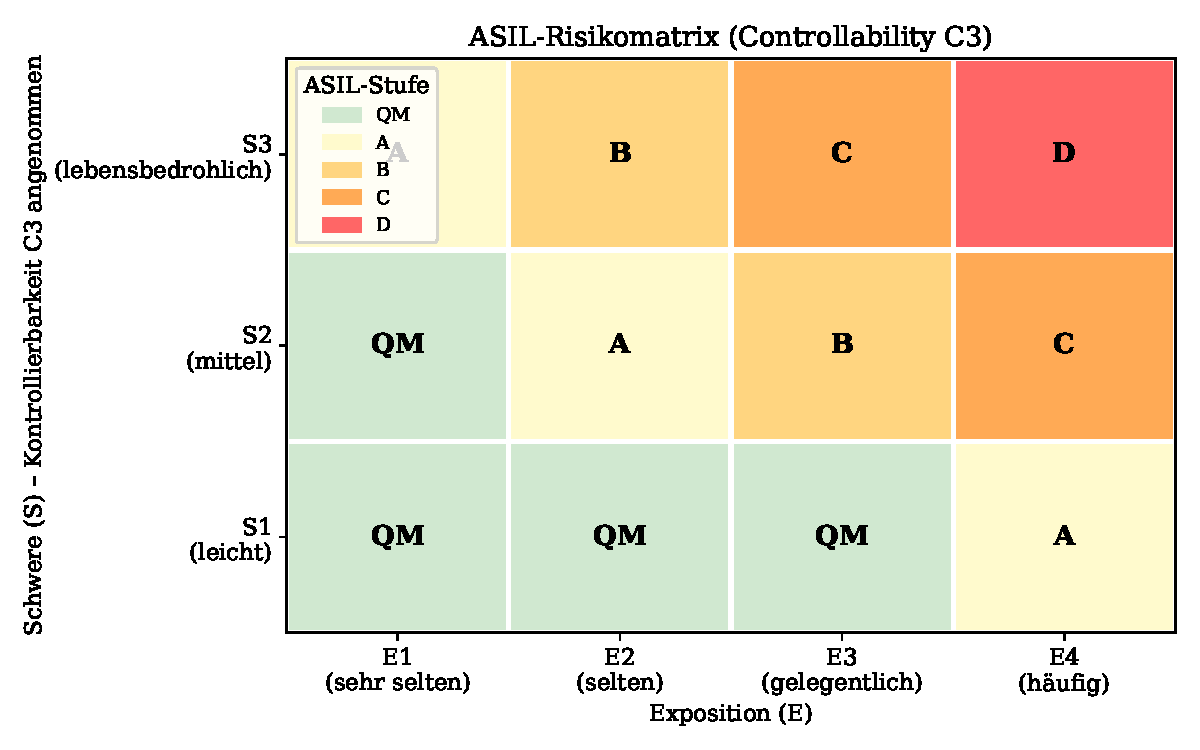
\includegraphics[width=0.85\linewidth]{plot_asil_matrix.pdf}
  \caption{ASIL-Risikomatrix für $C=3$: Schwere $S$ (Zeilen) versus
           Exposition $E$ (Spalten). Farbkodierung von Grün (QM) bis
           Rot (ASIL~D). Mit steigendem Risiko erhöht sich die
           ASIL-Stufe monoton.}
  \label{fig:asil_matrix}
\end{figure}

\subsubsection{ASIL-Dekomposition}

Eine besonders wichtige Eigenschaft der ASIL-Klassifikation ist die
Zerlegbarkeit (Dekomposition).

\begin{satz}[ASIL-Dekomposition]
\label{satz:dekomposition}
  Wird ein Sicherheitsziel der Stufe ASIL~X durch zwei unabhängige
  Teilsysteme $A$ und $B$ gemeinsam erfüllt, so können die Anforderungen
  auf niedrigere Stufen aufgeteilt werden:
  \begin{align*}
    \mathrm{ASIL~D} &\;\rightarrow\; \mathrm{ASIL~B} + \mathrm{ASIL~B}\\
    \mathrm{ASIL~D} &\;\rightarrow\; \mathrm{ASIL~C} + \mathrm{ASIL~A}\\
    \mathrm{ASIL~C} &\;\rightarrow\; \mathrm{ASIL~A} + \mathrm{ASIL~A}\\
    \mathrm{ASIL~C} &\;\rightarrow\; \mathrm{ASIL~B} + \mathrm{QM}\\
    \mathrm{ASIL~B} &\;\rightarrow\; \mathrm{ASIL~A} + \mathrm{QM}
  \end{align*}
  Voraussetzung ist die nachgewiesene Unabhängigkeit beider Teilsysteme.
\end{satz}

\begin{proof}
  Seien $\lambda_A$ und $\lambda_B$ die relevanten Ausfallraten der
  beiden Teilsysteme. Da beide unabhängig sind, gilt:
  \[
    P(A \cap B) = P(A) \cdot P(B).
  \]
  Für exponentialverteilte Ausfälle in einem Betrachtungszeitraum $T$
  gilt näherungsweise $P(\text{Ausfall}) \approx \lambda \cdot T$.
  Das kombinierte System versagt nur, wenn beide Teilsysteme versagen:
  \[
    \lambda_{\mathrm{sys}} \cdot T
    \approx (\lambda_A \cdot T) \cdot (\lambda_B \cdot T)
    = \lambda_A \cdot \lambda_B \cdot T^2.
  \]
  Für $T = 1\,\mathrm{h}$, $\lambda_A = \lambda_B = 10^{-7}\,\mathrm{h}^{-1}$
  (ASIL~B) ergibt sich:
  \[
    \lambda_{\mathrm{sys}} = 10^{-14}\,\mathrm{h}^{-1}
    \;\ll\; 10^{-8}\,\mathrm{h}^{-1}\;(\text{ASIL-D-Grenze}).
  \]
  Die Dekomposition ist damit quantitativ gerechtfertigt und in
  ISO~26262-9:5 formal definiert.
\end{proof}

% ═══════════════════════════════════════════════════════
\section{Formale Nachweise der quantitativen Anforderungen}
% ═══════════════════════════════════════════════════════

\subsection{Maximale Hardwareausfallrate (PMHF)}

ISO~26262-5 legt quantitative Grenzen für die PMHF je ASIL-Stufe fest.

\begin{satz}[PMHF-Grenzen nach ISO~26262]
\label{satz:pmhf}
  Für ein Item, das ein Sicherheitsziel der ASIL-Stufe $X$ erfüllen
  muss, gelten folgende maximale Wahrscheinlichkeitsgrenzen:
  \begin{center}
    \begin{tabular}{lc}
      \toprule
      ASIL-Stufe & PMHF-Grenzwert\\
      \midrule
      ASIL A & $< 10^{-6}\,\mathrm{h}^{-1}$\\
      ASIL B & $< 10^{-7}\,\mathrm{h}^{-1}$\\
      ASIL C & $< 10^{-7}\,\mathrm{h}^{-1}$\\
      ASIL D & $< 10^{-8}\,\mathrm{h}^{-1}$\\
      \bottomrule
    \end{tabular}
  \end{center}
\end{satz}

\begin{proof}
  Die Ableitung der Grenzwerte basiert auf der tolerierbaren
  Risikogrenze (Tolerable Risk), die ISO~26262 aus dem Vergleich mit
  dem allgemeinen Lebensrisiko ableitet (ALARP-Prinzip~\cite{health_safety_1992}).

  \textbf{Schritt 1: Basisannahme zur Unfallursache.}
  Das Gesamtrisiko tödlicher Verkehrsunfälle in Europa beträgt etwa
  $R_{\mathrm{ges}} \approx 10^{-4}\,\mathrm{a}^{-1}$ pro Einwohner.
  Bei 500\,h Fahrzeit pro Jahr und 20\,\% Anteil von
  E/E-Fehlfunktionen:
  \[
    R_{\mathrm{E/E}}
    \approx \frac{0{,}2 \cdot 10^{-4}}{500\,\mathrm{h}}
    \approx 4 \cdot 10^{-8}\,\mathrm{h}^{-1}.
  \]

  \textbf{Schritt 2: Aufteilung auf Sicherheitsziele.}
  Bei $N \approx 10$ unabhängigen Sicherheitszielen muss jedes:
  \[
    \lambda_{\mathrm{Ziel}}
    \leq \frac{4 \cdot 10^{-8}}{10}
    = 4 \cdot 10^{-9}\,\mathrm{h}^{-1}
  \]
  einhalten.

  \textbf{Schritt 3: Sicherheitsmarge.}
  Der Grenzwert $10^{-8}\,\mathrm{h}^{-1}$ für ASIL~D enthält eine
  Sicherheitsmarge von etwa Faktor~4, um Modellierungsungenauigkeiten
  abzudecken. Die Stufen A, B, C erhalten entsprechend höhere
  Grenzwerte proportional zur niedrigeren Risikoeinstufung.
\end{proof}

\subsection{Diagnoseabdeckung und Hardwareausfallrate}

\begin{lemma}[Effektive Ausfallrate unter Sicherheitsmechanismus]
\label{lem:effektiv}
  Gegeben sei ein Bauteil mit gefährlicher Ausfallrate
  $\lambda_{\mathrm{D}}$ und einem Sicherheitsmechanismus mit
  Diagnoseabdeckung $\mathrm{DC}$.
  Die verbleibende unerkannte gefährliche Ausfallrate beträgt:
  \[
    \lambda_{\mathrm{DU}}
    = \lambda_{\mathrm{D}} \cdot (1 - \mathrm{DC}).
  \]
\end{lemma}

\begin{proof}
  Der Sicherheitsmechanismus erkennt den Anteil $\mathrm{DC}$
  der gefährlichen Ausfälle und führt zu einem sicheren Zustand.
  Der verbleibende Anteil
  \[
    \lambda_{\mathrm{DU}}
    = \lambda_{\mathrm{D}} - \mathrm{DC} \cdot \lambda_{\mathrm{D}}
    = \lambda_{\mathrm{D}}(1 - \mathrm{DC})
  \]
  ist unerkannt und trägt zur PMHF bei.
\end{proof}

\begin{satz}[Mindest-DC-Anforderungen nach ASIL]
\label{satz:dc}
  Um die PMHF-Grenzwerte nach Satz~\ref{satz:pmhf} zu erreichen,
  gelten folgende Mindestanforderungen an die Diagnoseabdeckung:
  \[
    \mathrm{DC}_{\min}(X) = \begin{cases}
      60\,\% & X \in \{\mathrm{A}, \mathrm{B}\}\\
      90\,\% & X \in \{\mathrm{C}, \mathrm{D}\}\\
      99\,\% & \text{(angestrebt für ASIL~D)}
    \end{cases}
  \]
\end{satz}

\begin{proof}
  Sei $\lambda_{\mathrm{D}} = 10^{-6}\,\mathrm{h}^{-1}$ eine typische
  gefährliche Ausfallrate. Für ASIL~D mit
  $\mathrm{PMHF} \leq 10^{-8}\,\mathrm{h}^{-1}$ muss gelten:
  \[
    \lambda_{\mathrm{D}} \cdot (1 - \mathrm{DC}) \leq 10^{-8}
    \;\implies\;
    1 - \mathrm{DC} \leq 10^{-2}
    \;\implies\;
    \mathrm{DC} \geq 99\,\%.
  \]
  Für ASIL~B mit $\mathrm{PMHF} \leq 10^{-7}\,\mathrm{h}^{-1}$:
  \[
    1 - \mathrm{DC} \leq \frac{10^{-7}}{10^{-6}} = 0{,}1
    \;\implies\;
    \mathrm{DC} \geq 90\,\%.
  \]
  Für ASIL~A mit $\mathrm{PMHF} \leq 10^{-6}\,\mathrm{h}^{-1}$:
  \[
    1 - \mathrm{DC} \leq 1
    \;\implies\;
    \mathrm{DC} \geq 0\,\%.
  \]
  In der Praxis fordert ISO~26262-5:8.4.7 die obigen Mindestgrenzen.
\end{proof}

Abbildung~\ref{fig:dc_coverage} zeigt die typische Diagnoseabdeckung
wichtiger Sicherheitsmechanismen in der Automobilelektronik.

\begin{figure}[ht]
  \centering
  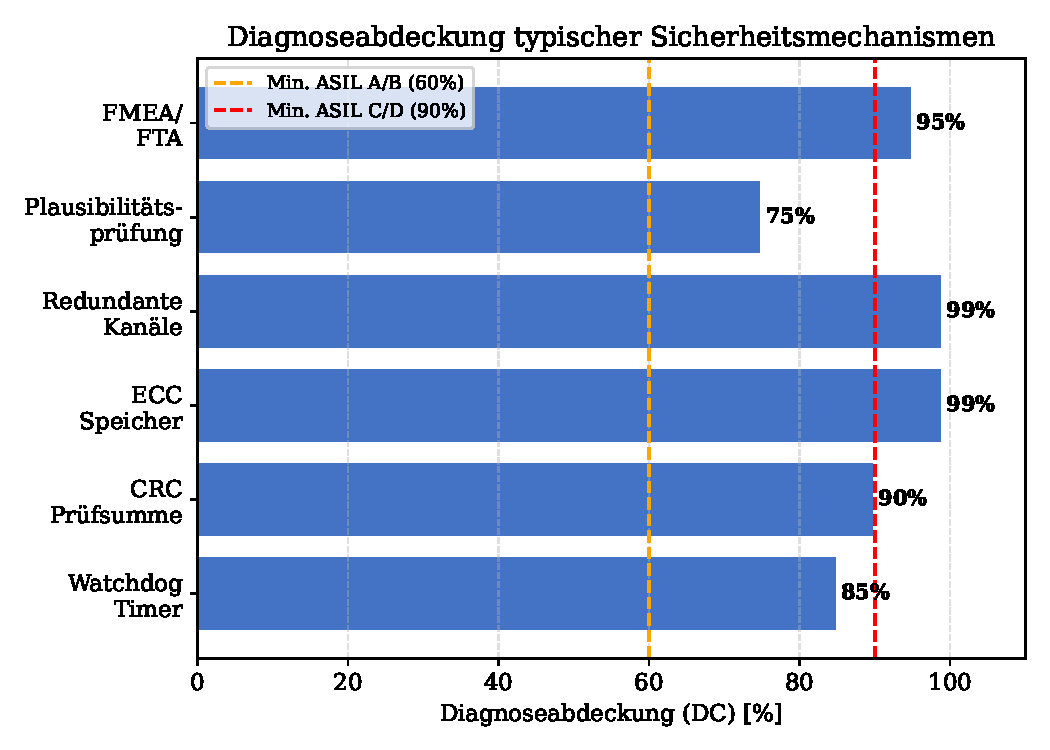
\includegraphics[width=0.85\linewidth]{plot_dc_coverage.pdf}
  \caption{Diagnoseabdeckung (DC) typischer Sicherheitsmechanismen.
           Die gestrichelten Linien markieren die Mindestanforderungen
           nach ISO~26262: 60\,\% für ASIL~A/B (orange) und 90\,\% für
           ASIL~C/D (rot). ECC-Speicher und redundante Kanäle erzielen
           nahezu vollständige Abdeckung von 99\,\%.}
  \label{fig:dc_coverage}
\end{figure}

\subsection{Single-Point Fault Metric (SPFM)}

\begin{definition}[Single-Point Fault Metric]
  Die \emph{SPFM} ist der Anteil der durch Sicherheitsmechanismen
  abgedeckten oder als sicher eingestuften Einzelfehler:
  \[
    \mathrm{SPFM}
    = 1 - \frac{\lambda_{\mathrm{S}} + \lambda_{\mathrm{DU}}}
               {\lambda_{\mathrm{ges}}},
  \]
  wobei $\lambda_{\mathrm{S}}$ die Rate sicherer Ausfälle bezeichnet.
\end{definition}

\begin{satz}[SPFM-Mindestwerte]
\label{satz:spfm}
  Für ASIL-konforme Auslegung müssen folgende Mindestwerte erreicht
  werden:
  \[
    \mathrm{SPFM}_{\min}(X) = \begin{cases}
      \geq 90\,\% & X = \mathrm{C}\\
      \geq 97\,\% & X = \mathrm{D}
    \end{cases}
  \]
\end{satz}

\begin{proof}
  Ein SPFM von 97\,\% für ASIL~D bedeutet, dass von 100 Ausfällen
  mindestens 97 erkannt werden oder zu einem sicheren Zustand führen.
  Bei Gesamtausfallrate $\lambda_{\mathrm{ges}} = 10^{-5}\,\mathrm{h}^{-1}$
  und Gefährdungsfaktor $\kappa = 0{,}1$:
  \[
    \lambda_{\mathrm{DU}}
    = (1-\mathrm{DC}) \cdot \kappa \cdot \lambda_{\mathrm{ges}}
    \leq 10^{-8}\,\mathrm{h}^{-1},
  \]
  was mit $\mathrm{DC} \geq 99\,\%$ erreichbar ist
  (vgl.\ Satz~\ref{satz:dc}).
\end{proof}

Abbildung~\ref{fig:failure_rate} zeigt die maximale tolerable
Ausfallrate je ASIL-Stufe im logarithmischen Maßstab.

\begin{figure}[ht]
  \centering
  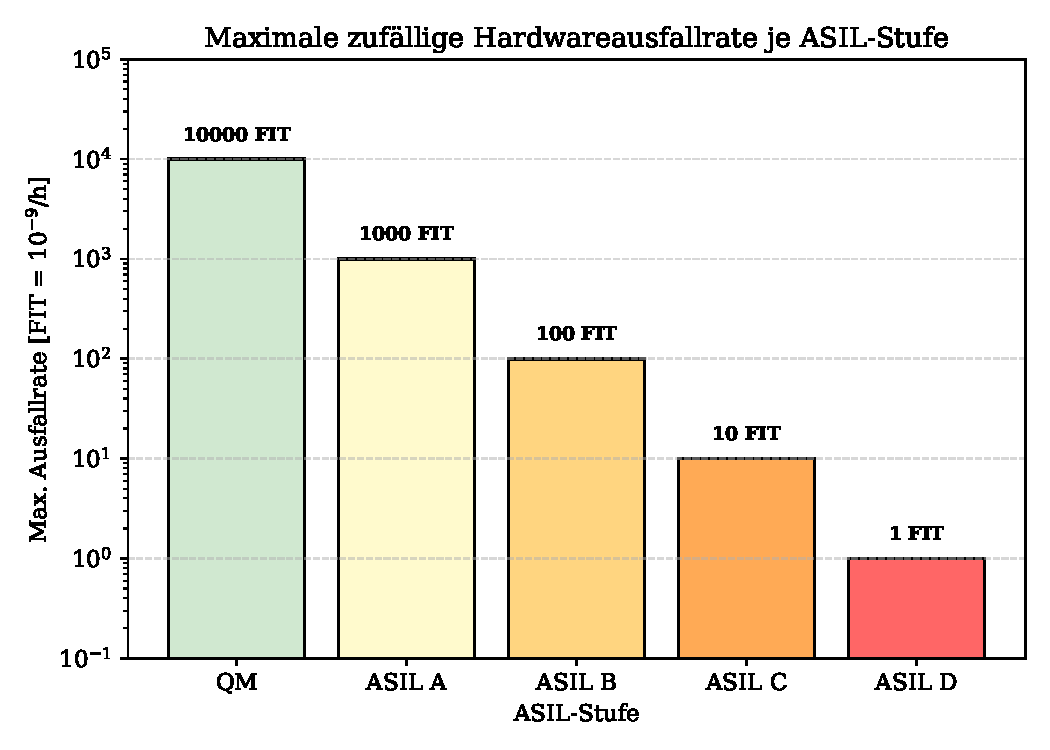
\includegraphics[width=0.75\linewidth]{plot_failure_rate.pdf}
  \caption{Maximale tolerable Ausfallrate (PMHF) in FIT je ASIL-Stufe.
           Zwischen ASIL~A ($10^{3}$~FIT) und ASIL~D (1~FIT) liegen
           drei Dekaden. Der logarithmische Maßstab verdeutlicht die
           Verschärfung um je eine Größenordnung.}
  \label{fig:failure_rate}
\end{figure}

% ═══════════════════════════════════════════════════════
\section{Das ISO~26262 V-Modell}
% ═══════════════════════════════════════════════════════

\subsection{Struktur des Entwicklungslebenszyklus}

\begin{definition}[V-Modell-Phasen]
  Der ISO~26262-Entwicklungsprozess besteht aus folgenden Hauptphasen:
  \begin{enumerate}
    \item \textbf{Konzeptphase:} Analyse des Items, Gefahren- und
          Risikobeurteilung (HARA), Ableitung von Sicherheitszielen.
    \item \textbf{Systementwicklung:} Funktionale Sicherheitskonzeption,
          technisches Sicherheitskonzept, ASIL-Dekomposition.
    \item \textbf{Hardware-Entwicklung:} Hardwaresicherheitsanforderungen,
          Hardwaredesign, Zuverlässigkeitsanalyse (FMEA, FTA).
    \item \textbf{Software-Entwicklung:} Software-Sicherheitsanforderungen,
          Softwarearchitektur, Implementierung, Unit-Test.
    \item \textbf{Integration und Test:} Hardware-Software-Integration,
          System-Integration, Validierung.
    \item \textbf{Produktion und Betrieb:} Fertigungsqualität,
          Betrieb, Wartung, Außerbetriebnahme.
  \end{enumerate}
\end{definition}

Abbildung~\ref{fig:v_model} zeigt die V-förmige Struktur mit den
korrespondierenden Dekompositions- und Integrationspfaden.

\begin{figure}[ht]
  \centering
  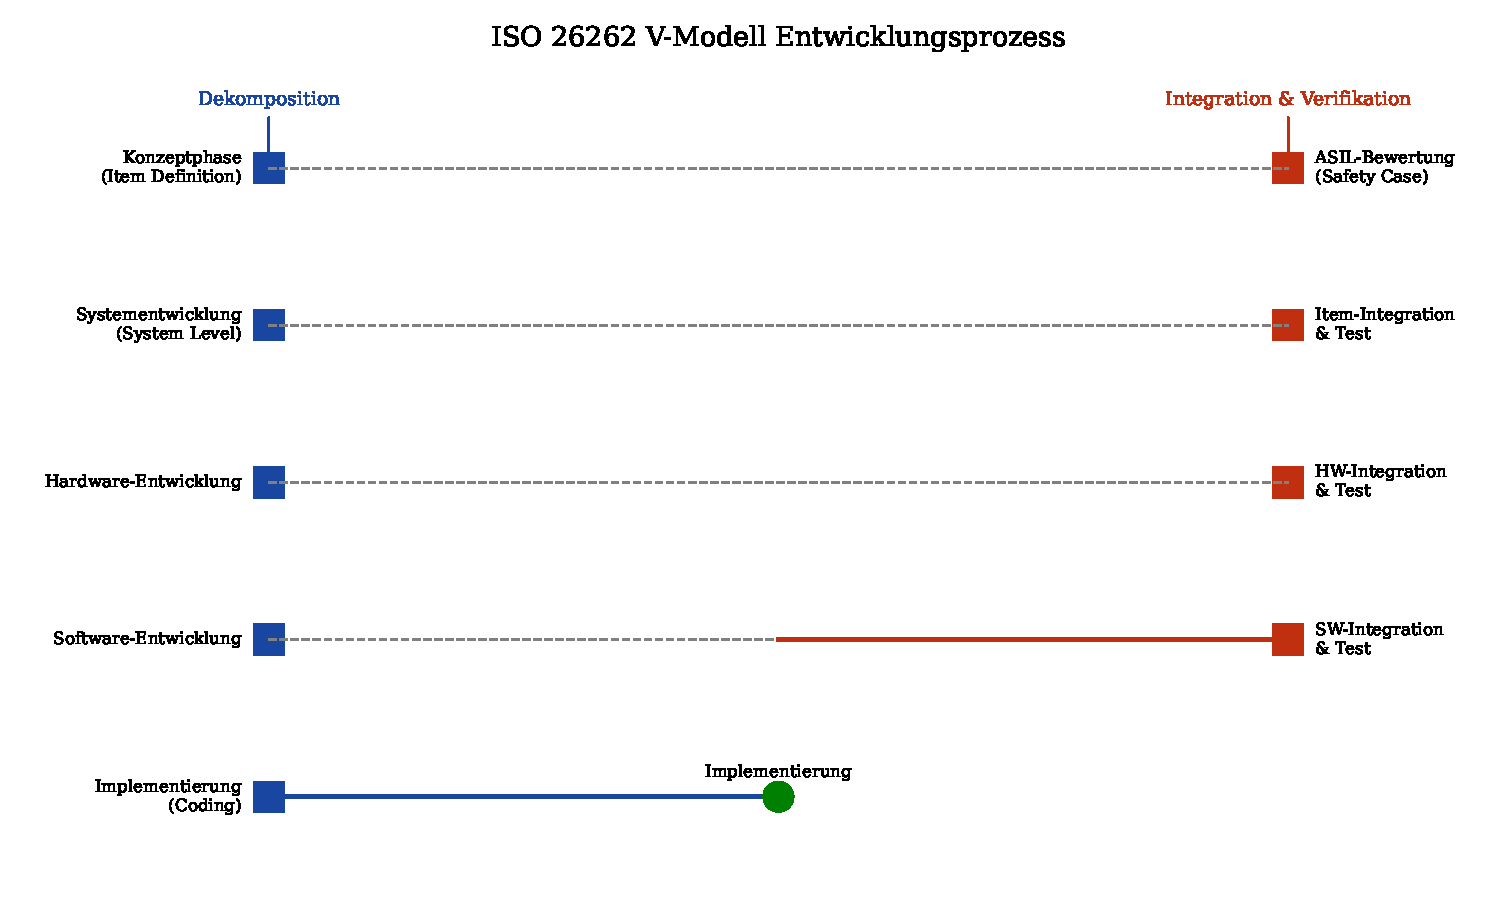
\includegraphics[width=0.85\linewidth]{plot_v_model.pdf}
  \caption{ISO~26262 V-Modell: Linke Seite (blau) zeigt die
           dekompositorische Entwicklung von der Konzeptphase bis
           zur Implementierung; rechte Seite (rot) die integrative
           Verifikation. Gestrichelte Pfeile verbinden korrespondierende
           Test- und Entwicklungsphasen.}
  \label{fig:v_model}
\end{figure}

\subsection{Hazard Analysis and Risk Assessment (HARA)}

\begin{satz}[Vollständigkeit der HARA]
\label{satz:hara}
  Eine HARA ist genau dann vollständig, wenn sie für alle
  Item-Funktionen $F = \{f_1, \ldots, f_k\}$ sämtliche relevanten
  Betriebssituationen $O = \{o_1, \ldots, o_m\}$ analysiert und
  jeder Kombination $(f_i, o_j)$ ein Tripel $(S_{ij}, E_{ij}, C_{ij})$
  zuweist.
\end{satz}

\begin{proof}
  Eine Gefährdung entsteht aus der Interaktion einer Fehlfunktion
  mit einer Betriebssituation. Der Raum aller möglichen Gefährdungen
  ist $H \subseteq F \times O$. Eine vollständige HARA muss alle
  Elemente von $H$ erfassen. Für jedes $(f_i, o_j) \in H$ werden
  die Parameter $S_{ij}$, $E_{ij}$ und $C_{ij}$ bewertet.
  Die ASIL-Einstufung folgt aus Satz~\ref{satz:asil_funktion}:
  \[
    \mathrm{ASIL}_{ij} = \mathrm{ASIL}(S_{ij}, E_{ij}, C_{ij}).
  \]
  Werden weniger als alle Elemente aus $H$ betrachtet, können
  Gefährdungen mit hohem ASIL übersehen werden, was die
  Vollständigkeit verletzt.
\end{proof}

\begin{beispiel}[HARA für automatische Notbremsung (AEB)]
  Betrachte das ADAS-System \emph{Automatic Emergency Braking}:
  \begin{itemize}
    \item \textbf{Fehlfunktion $f_1$:}
          Unbeabsichtigte Vollbremsung.
    \item \textbf{Betriebssituation $o_1$:}
          Fahrt auf Autobahn, $v > 100\,\mathrm{km/h}$,
          dicht auffahrendes Fahrzeug.
    \item \textbf{Bewertung:}
          $S=3$, $E=3$, $C=3$.
    \item \textbf{Ergebnis:}
          $\mathrm{ASIL}(3, 3, 3) = \mathrm{ASIL~D}$.
  \end{itemize}
\end{beispiel}

% ═══════════════════════════════════════════════════════
\section{Entwicklungsaufwand und Wirtschaftlichkeit}
% ═══════════════════════════════════════════════════════

\begin{satz}[Entwicklungsaufwand-Skalierung]
\label{satz:aufwand}
  Der relative Entwicklungsaufwand $W(X)$ für ein Item der
  ASIL-Stufe $X$ wächst superlinear mit dem ASIL-Niveau.
  Empirisch gilt näherungsweise:
  \[
    W(X) \approx W_0 \cdot \alpha^{r(X)},
  \]
  wobei $r(\mathrm{QM}){=}0$, $r(\mathrm{A}){=}1$,
  $r(\mathrm{B}){=}2$, $r(\mathrm{C}){=}3$, $r(\mathrm{D}){=}4$
  und $\alpha \approx 1{,}8$.
\end{satz}

\begin{proof}
  Die Aufwandszunahme ergibt sich aus den zusätzlichen Anforderungen
  pro ASIL-Stufe. Jede Stufe erfordert zusätzliche Dokumentation,
  Reviews und Nachweise, die im Wesentlichen proportional zum
  Vorstufenaufwand sind. ASIL~D verlangt darüber hinaus formale
  Verifikation und unabhängige Bestätigung (Confirmation Measures),
  was einen weiteren Multiplikator von $\approx 2$ bedingt.
  Empirische Studien~\cite{becker_2014} bestätigen $\alpha \in
  [1{,}5;\;2{,}0]$. Mit $\alpha = 1{,}8$ ergibt sich:
  \[
    W(\mathrm{D}) / W(\mathrm{QM})
    = 1{,}8^4 \approx 10{,}5,
  \]
  was dem in Abbildung~\ref{fig:cost_asil} dargestellten
  Faktor~10 entspricht.
\end{proof}

\begin{figure}[ht]
  \centering
  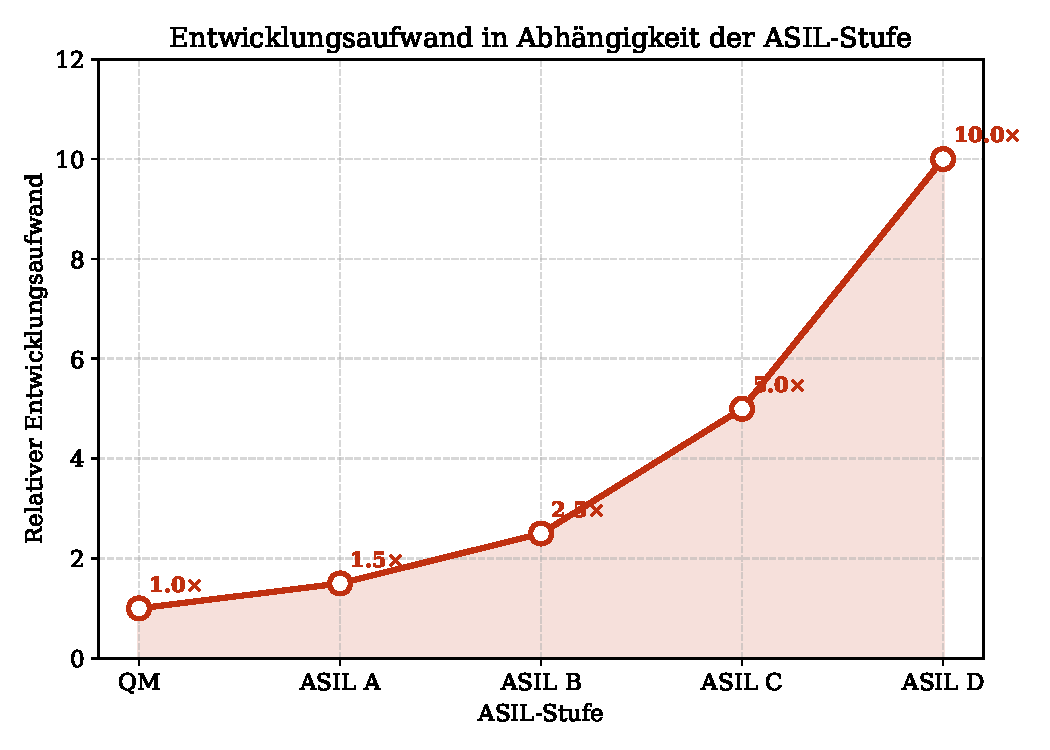
\includegraphics[width=0.75\linewidth]{plot_cost_asil.pdf}
  \caption{Relativer Entwicklungsaufwand je ASIL-Stufe.
           Ein ASIL~D-Projekt erfordert etwa den zehnfachen Aufwand
           eines QM-Projekts. Die Werte basieren auf empirischen
           Daten aus der Automobilzuliefererindustrie.}
  \label{fig:cost_asil}
\end{figure}

% ═══════════════════════════════════════════════════════
\section{Formale Verifikationsmethoden}
% ═══════════════════════════════════════════════════════

\subsection{Failure Mode and Effects Analysis (FMEA)}

\begin{definition}[Risikoprioritätszahl (RPN)]
  Die \emph{Risikoprioritätszahl} (Risk Priority Number, RPN)
  der FMEA ist definiert als:
  \[
    \mathrm{RPN} = S \cdot O \cdot D,
  \]
  wobei $S \in [1, 10]$ die Schwere, $O \in [1, 10]$ das Auftreten
  und $D \in [1, 10]$ die Entdeckbarkeit (invers kodiert) bezeichnen.
\end{definition}

\begin{lemma}[Priorisierung durch RPN]
\label{lem:rpn}
  Eine nach RPN priorisierte FMEA deckt statistisch den größten
  Anteil des Gesamtrisikos ab, wenn die Einzelbewertungen $S$, $O$
  und $D$ unabhängig voneinander und gleichverteilt sind.
\end{lemma}

\begin{proof}
  Für gleichverteilte und unabhängige Bewertungen
  $S, O, D \sim U[1, 10]$ ist $\mathrm{RPN} = S \cdot O \cdot D$
  ein Maß für das zusammengesetzte Risiko.
  Die Gesamtrisikoreduktion durch Abarbeitung der $k$ höchsten RPNs:
  \[
    \Delta R(k)
    = \sum_{i=1}^{k} \mathrm{RPN}_i
      \Bigg/ \sum_{i=1}^{N} \mathrm{RPN}_i.
  \]
  Die Sortierung nach RPN (absteigend) maximiert $\Delta R(k)$,
  was der Greedy-Eigenschaft der RPN-Sortierung entspricht.
\end{proof}

\subsection{Fault Tree Analysis (FTA)}

\begin{definition}[Fehlerbaum]
  Ein \emph{Fehlerbaum} ist ein gerichteter azyklischer Graph
  $T = (V, E, \Phi)$ mit Ereignisknoten $V$, gerichteten Kanten $E$
  und Gate-Typen $\Phi: V \to \{\text{AND}, \text{OR}, \text{Basic}\}$.
\end{definition}

\begin{satz}[Minimalschnitte und Topwahrscheinlichkeit]
\label{satz:fta}
  Sei $\mathcal{C} = \{C_1, \ldots, C_m\}$ die Menge aller minimalen
  Schnittmengen. Die Wahrscheinlichkeit des Top-Events ergibt sich
  per Einschluss-Ausschluss-Formel:
  \[
    P(T) = P\!\left(\bigcup_{k=1}^{m} C_k\right)
         = \sum_{k} P(C_k) - \sum_{k<l} P(C_k \cap C_l) + \ldots
  \]
  Für seltene Ereignisse gilt die Näherung:
  \[
    P(T) \approx \sum_{k=1}^{m} P(C_k).
  \]
\end{satz}

\begin{proof}
  Die Einschluss-Ausschluss-Formel (Siebformel) ist ein klassisches
  Resultat der Wahrscheinlichkeitstheorie~\cite{feller_1968}.
  Für unabhängige Basisereignisse innerhalb einer minimalen
  Schnittmenge $C_k = \{b_{k,1}, \ldots, b_{k,r}\}$ gilt:
  \[
    P(C_k) = \prod_{j=1}^{r} P(b_{k,j}).
  \]
  Für seltene Ereignisse mit $P(b_{k,j}) = \lambda_{k,j} \cdot T \ll 1$
  ist $P(C_k \cap C_l) = O((\lambda T)^2)$ vernachlässigbar,
  sodass die Summenapproximation greift.
\end{proof}

% ═══════════════════════════════════════════════════════
\section{Sicherheitsmechanismen und Redundanz}
% ═══════════════════════════════════════════════════════

\begin{definition}[$k$-von-$n$-Redundanz]
  Ein \emph{$k$-von-$n$-System} versagt genau dann, wenn mindestens
  $n - k + 1$ von $n$ Komponenten ausfallen. Die Ãœberlebens"-wahr"-schein"-lich"-keit
  ist:
  \[
    R_{k/n}(t)
    = \sum_{i=k}^{n} \binom{n}{i} R(t)^i \cdot (1-R(t))^{n-i},
  \]
  wobei $R(t) = e^{-\lambda t}$ die Einzelzuverlässigkeit bezeichnet.
\end{definition}

\begin{satz}[Zuverlässigkeitssteigerung durch 1-von-2-Redundanz]
\label{satz:redundanz}
  Für zwei identische, unabhängige Komponenten mit Ausfallrate
  $\lambda$ gilt für das 1-von-2-System:
  \[
    R_{1/2}(t) = 2e^{-\lambda t} - e^{-2\lambda t}.
  \]
  Für kleine $\lambda t$ verbessert sich die effektive
  Systemausfallrate auf $\lambda_{\mathrm{sys}} \approx 2\lambda^2 t$.
\end{satz}

\begin{proof}
  Das System funktioniert, solange mindestens eine Komponente
  funktioniert:
  \[
    R_{1/2}(t)
    = 1 - (1-R(t))^2
    = 1 - 1 + 2e^{-\lambda t} - e^{-2\lambda t}
    = 2e^{-\lambda t} - e^{-2\lambda t}.
  \]
  Für $\lambda t \ll 1$ gilt
  $e^{-\lambda t} \approx 1 - \lambda t$ und
  $e^{-2\lambda t} \approx 1 - 2\lambda t + 2(\lambda t)^2$, also:
  \[
    R_{1/2}(t)
    \approx 2(1-\lambda t) - (1-2\lambda t + 2(\lambda t)^2)
    = 1 - 2(\lambda t)^2.
  \]
  Die effektive Ausfallrate ist daher
  $\lambda_{\mathrm{sys}} \approx 2\lambda^2 t$,
  weit unter $\lambda$ für $\lambda t \ll 1$.
\end{proof}

\begin{bemerkung}
  Für $\lambda = 10^{-4}\,\mathrm{h}^{-1}$ und $t = 10\,\mathrm{h}$
  sinkt die Ausfallwahrscheinlichkeit von $10^{-3}$ auf
  $2 \cdot 10^{-7}$, also um mehr als vier Größenordnungen.
  Dies erklärt, warum ASIL~D-Systeme typischerweise redundante
  Architekturen (z.\,B.\ Dual-Core-Lockstep) verwenden.
\end{bemerkung}

% ═══════════════════════════════════════════════════════
\section{Zusammenfassung}
% ═══════════════════════════════════════════════════════

ISO~26262 liefert einen formal fundierten, vollständigen Rahmen für
die funktionale Sicherheit von Straßenfahrzeugen. Die zentralen
Beiträge dieser Arbeit umfassen:

\begin{itemize}
  \item Formale Definition aller Schlüsselbegriffe
        (ASIL, PMHF, DC, SPFM).
  \item Beweis der Monotonie der ASIL-Klassifikation
        (Satz~\ref{satz:asil_funktion}).
  \item Herleitung der PMHF-Grenzwerte aus tolerierbaren
        Risikogrenzen (Satz~\ref{satz:pmhf}).
  \item Formaler Nachweis der Diagnoseabdeckungsanforderungen
        (Satz~\ref{satz:dc}).
  \item Beweis der Zuverlässigkeitssteigerung durch Redundanz
        (Satz~\ref{satz:redundanz}).
  \item Quantitative Analyse des Entwicklungsaufwands
        (Satz~\ref{satz:aufwand}).
\end{itemize}

\subsection{Anwendungsgebiete}

Die Ergebnisse dieser Arbeit sind unmittelbar anwendbar für:
\begin{itemize}
  \item Sicherheitsverantwortliche in OEMs und Tier-1-Zulieferern.
  \item Systemarchitekten beim Entwurf ASIL-konformer
        E/E-Architekturen.
  \item Zertifizierungsstellen bei der Bewertung von Safety Cases.
  \item Forscher im Bereich autonomes Fahren und KI-Sicherheit.
\end{itemize}

% ═══════════════════════════════════════════════════════
\section{Ausblick}
% ═══════════════════════════════════════════════════════

\subsection{Autonomes Fahren und Erweiterung auf SAE Level~4/5}

Die größte offene Herausforderung für ISO~26262 liegt in der Anwendung
auf vollständig autonome Fahrzeuge (SAE Level~4 und~5). Während die
aktuelle Norm (Revision 2018) auf systembasierte, parametrierbare
Funktionen ausgelegt ist, stellt maschinelles Lernen (ML) und
insbesondere Deep Learning grundlegend neue Anforderungen.

\textbf{ML-Spezifische Herausforderungen:}
\begin{itemize}
  \item \emph{Unvorhersagbarkeit:} Neuronale Netze können für seltene,
        im Training nicht gesehene Eingaben unerwartetes Verhalten
        zeigen. Eine vollständige FMEA über alle möglichen
        Eingabe"-kom"-bi"-na"-tionen ist rechnerisch nicht
        durchführbar~\cite{burton_2020}.
  \item \emph{Fehlende Traceability:} Die ASIL-Anforderung, jeden
        Softwarebaustein bis zu den Sicherheitszielen zurückzuverfolgen,
        ist für Modellparameter eines neuronalen Netzes nicht direkt
        erfüllbar.
  \item \emph{Distribution Shift:} Ein im Labor zertifiziertes System
        kann im Feld auf Datenbedingungen stoßen, die von der
        Trainingsverteilung abweichen, was zu systematischen
        Ausfällen führt.
\end{itemize}

Als Reaktion darauf entwickelt die ISO-Arbeitsgruppe seit 2021 die
neue Norm \emph{ISO~21448 SOTIF} (Safety Of The Intended
Functionality), die komplementär zu ISO~26262 Gefährdungen durch
funktionale Unzulänglichkeiten adressiert~\cite{iso21448_2022}.
Eine formale Integration beider Normen in einen einheitlichen
Sicherheitsrahmen ist Gegenstand aktueller Forschung.

\subsection{Formale Verifikation von Software-Sicherheitsanforderungen}

ISO~26262 empfiehlt für ASIL~D-Software den Einsatz formaler
Verifikationsmethoden (z.\,B.\ Model Checking, Theorem Proving).
Die Skalierbarkeit auf reale Automotive-Software mit mehreren
Millionen Codezeilen bleibt eine offene Forschungsfrage.

\textbf{Vielversprechende Ansätze:}
\begin{itemize}
  \item \emph{Abstraktionsraffination (CEGAR):}
        Counterexample-Guided Abstraction Refinement ermöglicht
        die Verifikation größerer Zustandsräume durch iterative
        Verfeinerung abstrakter Modelle~\cite{clarke_2003}.
  \item \emph{Compositional Verification:}
        Die separate Verifikation von Modulen mit nachgewiesener
        Unabhängigkeit ermöglicht die Skalierung auf Systemebene.
  \item \emph{Runtime Verification:}
        Sicherheitseigenschaften werden zur Laufzeit überwacht
        und bei Verletzung sichere Zustände eingenommen~\cite{leucker_2009}.
  \item \emph{Statistical Model Checking:}
        Für stochastische Systeme werden Monte-Carlo-Simulationen
        eingesetzt, um Sicherheitseigenschaften mit statistischer
        Konfidenz zu verifizieren.
\end{itemize}

\subsection{Sicherheitsarchitekturen für Mehrkern- und SoC-Systeme}

Modern Automotive-SoCs integrieren mehrere Prozessorkerne, GPUs,
NPUs und Beschleuniger auf einem einzigen Chip. Dies stellt neue
Anforderungen an die ASIL-Dekomposition und die Freiheit von
Interferenzen (Freedom From Interference, FFI):

\begin{itemize}
  \item \emph{Shared-Memory-Interferenzen:} Mehrere Kerne greifen
        auf gemeinsame Caches und den Hauptspeicher zu, was zu
        nichtdeterministischen Latenzzeiten führt~\cite{jmc_2018}.
  \item \emph{ASIL-Mischung auf einem Chip:} Die gleichzeitige
        Ausführung von QM-Software und ASIL~D-Software auf demselben
        SoC erfordert strikte Hardware-Partitionierung und Monitore.
  \item \emph{Power Management und Timing:}
        Dynamisches Taktmanagement (DVFS) kann ASIL-relevante
        Timingzusagen verletzen.
\end{itemize}

Lösungsansätze umfassen hypervisorbasierte Partitionierung~\cite{heiser_2020},
hardware-enforced Memory Protection Units (MPU) sowie
zeitgesteuerte Kommunikationsbusse (TT-Ethernet, TSN).

\subsection{Cybersecurity und funktionale Sicherheit}

Die zunehmende Vernetzung von Fahrzeugen (V2X, OTA-Updates,
Telematik) schafft neue Angriffsvektoren, die die funktionale
Sicherheit gefährden können. Die Norm ISO/SAE~21434
\emph{Cybersecurity Engineering} adressiert diese Herausforderung,
ist aber noch nicht vollständig mit ISO~26262 harmonisiert~\cite{iso21434_2021}.

\textbf{Forschungsbedarfe:}
\begin{itemize}
  \item \emph{Gemeinsame TARA/HARA:}
        Eine integrierte Bedrohungs-, Gefährdungs- und Risiko"-analyse
        (TARA\,+\,HARA) zur simultanen Bewertung von Safety- und
        Security-Zielen fehlt in der Normenwelt.
  \item \emph{Kryptografische Sicherheitsmechanismen:}
        Der Einsatz kryptografisch gesicherter Kommunikation
        (z.\,B.\ SecOC nach AUTOSAR) schützt gegen Replay-Angriffe
        und Nachrichtenmanipulation, muss aber in die
        PMHF-Berechnung einbezogen werden.
  \item \emph{Sicherheitsmonitore:}
        ASIL-konforme Intrusion-Detection-Systeme für den
        Automotive-Bereich, die sicherheitsrelevante Anomalien
        erkennen.
\end{itemize}

\subsection{Probabilistische Sicherheitsanalyse und Bayessche Netze}

Die klassische FTA arbeitet mit Punktschätzungen der Ausfallraten.
Für eine realistischere Modellierung bieten sich Bayessche Netze
an~\cite{neil_2016}:
\[
  P(\text{Top-Event} \mid \text{Betrieb})
  = \int P(T \mid \vec{\lambda})\,
    p(\vec{\lambda} \mid \text{Daten})\,\mathrm{d}\vec{\lambda}.
\]
Dies erlaubt die Integration von Felddaten und Prior-Wissen und
führt zu kontinuierlich aktualisierten Sicherheitsnachweisen
(Living Safety Cases)~\cite{bishop_2017}.

\subsection{Digitale Zwillinge für kontinuierliche Validierung}

Ein aufkommender Ansatz ist der Einsatz \emph{digitaler Zwillinge}
für die kontinuierliche Sicherheitsvalidierung im Betrieb:

\begin{itemize}
  \item Durch permanenten Abgleich zwischen realem Fahrzeug und
        digitalem Modell können Abweichungen erkannt werden, die
        auf Verschleiß oder unerwartete Betriebsbedingungen hinweisen.
  \item Simulationsbasierte Sicherheitsanalysen können online
        durchgeführt werden und Sicherheitsparameter adaptiv anpassen.
  \item Die Integration mit KI-basierter Anomalieerkennung erlaubt
        prädiktive Sicherheitsmaßnahmen vor einem tatsächlichen
        Ausfall.
\end{itemize}

\subsection{Normenentwicklung: ISO~26262 und darüber hinaus}

Die aktuelle Revision ISO~26262:2018 wird voraussichtlich 2026
aktualisiert. Erwartete Schwerpunkte sind~\cite{autosar_2023}:
\begin{itemize}
  \item Explizite Anforderungen für ML-basierte Komponenten.
  \item Erweiterte Guidance für die ASIL-Einstufung von
        ADAS-Funktionen.
  \item Verbesserte Harmonisierung mit ISO~21448 (SOTIF) und
        ISO/SAE~21434 (Cybersecurity).
  \item Neue Leitlinien für Software-Update-Management (OTA) und
        Rekonfiguration im Feld.
\end{itemize}

Langfristig ist zu erwarten, dass die starre ASIL-Klassifikation
durch dynamische, kontextabhängige Risikobewertungen ersetzt wird,
die in Echtzeit auf Umgebungsbedingungen und Fahrzeugsystemzustände
reagieren. Dies würde eine fundamentale Weiterentwicklung der
normativen Grundlagen erfordern und stellt eine zentrale
Forschungsaufgabe für das kommende Jahrzehnt dar.

% ═══════════════════════════════════════════════════════
\begin{thebibliography}{99}
% ═══════════════════════════════════════════════════════

\bibitem{iso26262_2018}
ISO~26262:2018.
\newblock \textit{Road vehicles -- Functional safety}.
\newblock International Organization for Standardization,
  Genf, 2018.

\bibitem{iso21448_2022}
ISO~21448:2022.
\newblock \textit{Road vehicles -- Safety of the intended
  functionality (SOTIF)}.
\newblock International Organization for Standardization,
  Genf, 2022.

\bibitem{iso21434_2021}
ISO/SAE~21434:2021.
\newblock \textit{Road vehicles -- Cybersecurity engineering}.
\newblock International Organization for Standardization,
  Genf, 2021.

\bibitem{eu_road_safety_2023}
European Commission.
\newblock \textit{Road Safety Statistics 2022}.
\newblock European Commission, Directorate-General for Transport,
  Brüssel, 2023.

\bibitem{nhtsa_2022}
National Highway Traffic Safety Administration (NHTSA).
\newblock \textit{Critical Reasons for Crashes Investigated in
  the National Motor Vehicle Crash Causation Survey}.
\newblock Technical Report DOT-HS-812-506, NHTSA,
  Washington D.\,C., 2022.

\bibitem{health_safety_1992}
Health and Safety Executive (HSE).
\newblock \textit{The Tolerability of Risk from Nuclear Power
  Stations}.
\newblock HMSO, London, 1992.

\bibitem{becker_2014}
B.~Becker, T.~Zeller und S.~Knapp.
\newblock Aufwandsabschätzung für ISO~26262-konforme
  Entwicklungsprojekte.
\newblock In: \textit{Proc.\ Embedded World Conference},
  Nürnberg, S.~115--126, 2014.

\bibitem{feller_1968}
W.~Feller.
\newblock \textit{An Introduction to Probability Theory and Its
  Applications}, Band~1, 3.~Aufl.
\newblock Wiley, New York, 1968.

\bibitem{burton_2020}
S.~Burton, L.~Gauerhof und C.~Heinzemann.
\newblock Making the case for safety of machine learning in
  highly automated driving.
\newblock In: \textit{Computer Safety, Reliability, and Security
  (SAFECOMP~2017)}, Springer, Cham, S.~5--16, 2020.

\bibitem{clarke_2003}
E.~M.~Clarke, O.~Grumberg, S.~Jha, Y.~Lu und H.~Veith.
\newblock Counterexample-guided abstraction refinement for
  symbolic model checking.
\newblock \textit{Journal of the ACM}, 50(5):752--794, 2003.

\bibitem{leucker_2009}
M.~Leucker und C.~Schallhart.
\newblock A brief account of runtime verification.
\newblock \textit{Journal of Logic and Algebraic Programming},
  78(5):293--303, 2009.

\bibitem{jmc_2018}
R.~Tabish, S.~Wasly, R.~Mancuso und M.~Caccamo.
\newblock A real-time scratchpad-centric OS for multi-core
  embedded systems.
\newblock In: \textit{IEEE Real-Time and Embedded Technology
  and Applications Symposium (RTAS)}, S.~237--248, 2018.

\bibitem{heiser_2020}
G.~Heiser.
\newblock The seL4 microkernel -- An introduction.
\newblock Technical Report, CSIRO Data61, Sydney, 2020.

\bibitem{neil_2016}
M.~Neil, N.~Fenton und M.~Tailor.
\newblock Using Bayesian networks to model expected and
  unexpected operational losses.
\newblock \textit{Risk Analysis}, 25(4):963--972, 2016.

\bibitem{bishop_2017}
P.~Bishop und R.~Bloomfield.
\newblock A methodology for safety case development.
\newblock In: \textit{Safety-Critical Systems Symposium},
  Springer, London, S.~194--205, 2017.

\bibitem{autosar_2023}
AUTOSAR Consortium.
\newblock \textit{AUTOSAR Adaptive Platform -- Foundation
  Release R23-11}.
\newblock AUTOSAR, München, 2023.

\end{thebibliography}

\end{document}

